\noindent
\begin{minipage}[t]{0.25\textwidth}
    \vspace{0pt}
    \centering
    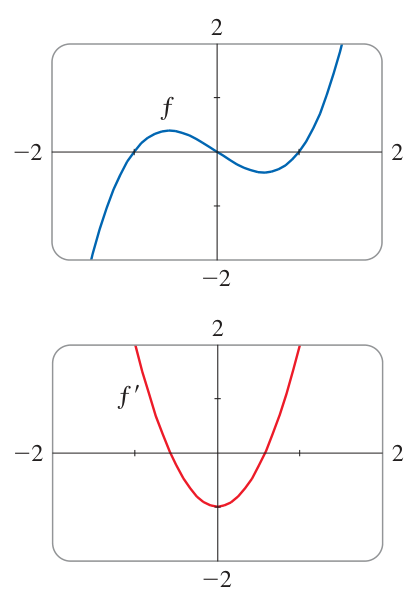
\includegraphics[width=\linewidth]{images/p0190_fig1.png}
    
    \vspace{4pt}
    \raggedright
    \noindent\textbf{\textsf{HÌNH 3}}
    
    \vspace{390pt}
    \noindent\textbf{\textsf{HÌNH 4}}
\end{minipage}%
\hfill
\begin{minipage}[t]{0.72\textwidth}
    \vspace{0pt}
    \noindent là $h$ và $x$ tạm thời được xem như một hằng số trong suốt quá trình tính giới hạn.
    \begin{align*}
        f'(x) &= \lim_{h \to 0} \frac{f(x+h) - f(x)}{h} = \lim_{h \to 0} \frac{[(x+h)^3 - (x+h)] - [x^3 - x]}{h} \\[6pt]
        &= \lim_{h \to 0} \frac{x^3 + 3x^2h + 3xh^2 + h^3 - x - h - x^3 + x}{h} \\[6pt]
        &= \lim_{h \to 0} \frac{3x^2h + 3xh^2 + h^3 - h}{h} \\[6pt]
        &= \lim_{h \to 0} (3x^2 + 3xh + h^2 - 1) = 3x^2 - 1
    \end{align*}

    \vspace{2pt}
    \noindent\textbf{(b)} Ta sử dụng máy tính cầm tay để vẽ đồ thị của $f$ và $f'$ trong Hình~3. Chú ý rằng $f'(x) = 0$ khi $f$ có các tiếp tuyến nằm ngang và $f'(x)$ mang giá trị dương khi các tiếp tuyến có hệ số góc dương. Do đó, các đồ thị này đóng vai trò như một phép kiểm tra lại kết quả của chúng ta ở câu~(a). \hfill{\color{stewartcyan}$\blacksquare$}

    \vspace{10pt}
    \noindent\textbf{\textsf{\color{stewartcyan}VÍ DỤ 3}}\hspace{1em}Nếu $f(x) = \sqrt{x}$, hãy tìm đạo hàm của $f$. Nêu rõ tập xác định của $f'$.

    \vspace{4pt}
    \noindent\textbf{\textsf{\color{stewartcyan}LỜI GIẢI}}
    \begin{align*}
        f'(x) &= \lim_{h \to 0} \frac{f(x+h) - f(x)}{h} = \lim_{h \to 0} \frac{\sqrt{x+h} - \sqrt{x}}{h} \\[6pt]
        &= \lim_{h \to 0} \left[ \frac{\sqrt{x+h} - \sqrt{x}}{h} \cdot \frac{\sqrt{x+h} + \sqrt{x}}{\sqrt{x+h} + \sqrt{x}} \right] \qquad \text{\color{stewartcyan}(Trục căn thức ở tử số.)} \\[6pt]
        &= \lim_{h \to 0} \frac{(x+h) - x}{h(\sqrt{x+h} + \sqrt{x})} = \lim_{h \to 0} \frac{h}{h(\sqrt{x+h} + \sqrt{x})} \\[6pt]
        &= \lim_{h \to 0} \frac{1}{\sqrt{x+h} + \sqrt{x}} = \frac{1}{\sqrt{x} + \sqrt{x}} = \frac{1}{2\sqrt{x}}
    \end{align*}

    \vspace{2pt}
    \noindent Ta thấy rằng $f'(x)$ tồn tại nếu $x > 0$, vì vậy tập xác định của $f'$ là $(0, \infty)$. Tập xác định này hẹp hơn một chút so với tập xác định của $f$, vốn là $[0, \infty)$. \hfill{\color{stewartcyan}$\blacksquare$}

    \vspace{8pt}
    \noindent\hspace*{14pt}Hãy kiểm tra xem kết quả của Ví dụ~3 có hợp lý hay không bằng cách quan sát đồ thị của $f$ và $f'$ trong Hình~4. Khi $x$ ở gần 0, $\sqrt{x}$ cũng ở gần 0, do đó $f'(x) = 1/(2\sqrt{x})$ rất lớn và điều này tương ứng với các tiếp tuyến rất dốc ở gần $(0, 0)$ trong Hình~4(a) cùng các giá trị lớn của $f'(x)$ ngay phía bên phải điểm 0 trong Hình~4(b). Khi $x$ lớn, $f'(x)$ rất nhỏ và điều này tương ứng với các đường tiếp tuyến phẳng hơn ở phía xa bên phải của đồ thị $f$ và đường tiệm cận ngang của đồ thị $f'$.

    \vspace{8pt}
    \begin{center}
        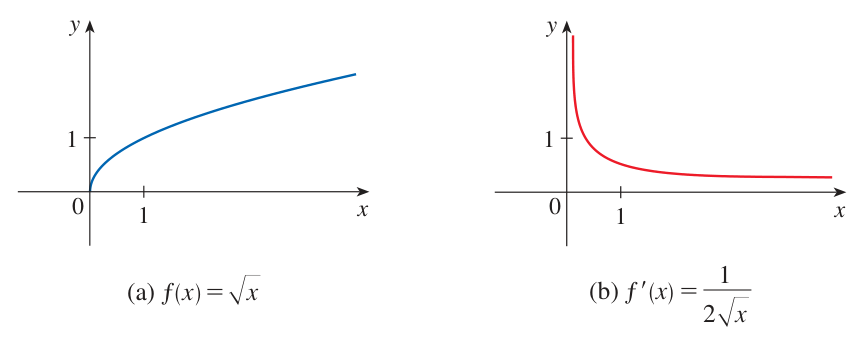
\includegraphics[width=0.96\linewidth]{images/p0190_fig2.png}
    \end{center}
\end{minipage}
